\documentclass[10pt]{article}
\usepackage[a4paper,margin=23mm]{geometry}
\usepackage{graphicx,booktabs,longtable,amsmath,url,microtype,float}
\renewcommand{\thetable}{S\arabic{table}}
\renewcommand{\thefigure}{S\arabic{figure}}
\renewcommand{\thesection}{S\arabic{section}}
\setcounter{tocdepth}{1}
\begin{document}
\begin{center}
{\Large Supplementary material}\par\medskip
Evaluating Crowd-Label Supervision for Selective Facial-Expression Recognition\par\medskip
SN Computer Science\par\smallskip
Gunjan Kumar Mishra, Bijaya Ghimire, Badri Raj Lamichhane, Alan Shah\par\smallskip
Corresponding author: Badri Raj Lamichhane\par
School of Information, Computer and Communication Technology,\par
Sirindhorn International Institute of Technology, Thammasat University, Thailand\par
\texttt{d6622300231@g.siit.tu.ac.th}
\end{center}
\section*{How to use this supplement}
Sections S1--S7 follow the seven Results subsections in the main article. Section S8 collects the fixed model architecture and the unvalidated messaging prototype. Section S9 records acquisition, annotation alignment, execution chronology and reproduction routes. Tables and figures provide the complete numerical diagnostics behind the main comparisons; the notation and uncertainty definitions are unchanged.

\tableofcontents
\medskip
\section*{Notation and interpretation}
Original numerical summaries are generated from \texttt{reported\_results.csv}. The additional score-sensitivity summaries are generated from the three \texttt{selector} CSV ledgers in the consolidated Online Resource 1.
S denotes Soft, U Uniform, H Hard, and T Tie-hard. Differences are percentage points.
The three seeds are fixed; they do not represent all possible retraining outcomes.
Training phases reuse one image source. A later analysis tests frozen models on acted videos and is reported separately. Neither analysis establishes a benefit for natural communication.
Global 80\% first selects images from the full population, then reports the retained images in each stratum. Within-stratum 80\% instead ranks and selects images separately inside that stratum.
Supported-only risk uses only votes for categories the model can predict. It is undefined when no votes fall in those categories.


\clearpage\section{Effects of supervision targets and checkpoint selection}\label{supp:targets}
\begin{longtable}{llrrr}
\caption{Original four-condition paired seed contrasts at 80\% coverage}\label{tab:seeds}\\
\toprule State & Contrast & Seed 17 & Seed 42 & Seed 89\\\midrule\endfirsthead
\toprule State & Contrast & Seed 17 & Seed 42 & Seed 89\\\midrule\endhead
selected & Soft - Uniform & -0.3473 & -0.4313 & -0.3550\\
selected & Soft - Hard & -2.1908 & -3.7328 & -1.9084\\
selected & Tie-hard - Hard & -0.0153 & -1.0992 & -0.2977\\
selected & Soft - Tie-hard & -2.1756 & -2.6336 & -1.6107\\
epoch12 & Soft - Uniform & -0.3282 & -0.3931 & -0.2290\\
epoch12 & Soft - Hard & -1.1794 & -1.4198 & -1.4542\\
epoch12 & Tie-hard - Hard & -0.2824 & -0.5076 & -0.4313\\
epoch12 & Soft - Tie-hard & -0.8969 & -0.9122 & -1.0229\\
\bottomrule\end{longtable}
Selected epochs for all five Swin conditions are consolidated in Table~\ref{tab:epochs}; every fixed-epoch sensitivity checkpoint is epoch 12.

\begin{table}[H]
\caption{Secondary matched Tie-Uniform comparison at 80\% coverage. Risks are percentages; differences and conditional 95\% intervals are percentage points}\label{tab:tieuniform}
\centering\begin{tabular}{lrrrr}\toprule
State & Tie-Uniform & Soft & Difference & Interval\\\midrule
selected & 24.272 & 23.684 & -0.588 & [-0.830, -0.281]\\
epoch12 & 23.939 & 23.632 & -0.307 & [-0.585, -0.024]\\
\bottomrule\end{tabular}\par

\end{table}

\begin{table}[H]
\caption{Selected epochs under the common distribution-distance criterion}\label{tab:epochs}
\centering\begin{tabular}{lrrr}\toprule
Targets & Seed 17 & Seed 42 & Seed 89\\\midrule
Hard & 3 & 2 & 5\\
Tie-hard & 4 & 4 & 5\\
Uniform & 9 & 6 & 10\\
Tie-Uniform & 12 & 8 & 7\\
Soft & 9 & 10 & 10\\
\bottomrule\end{tabular}\par

\end{table}

\begin{figure}[ht]
\centering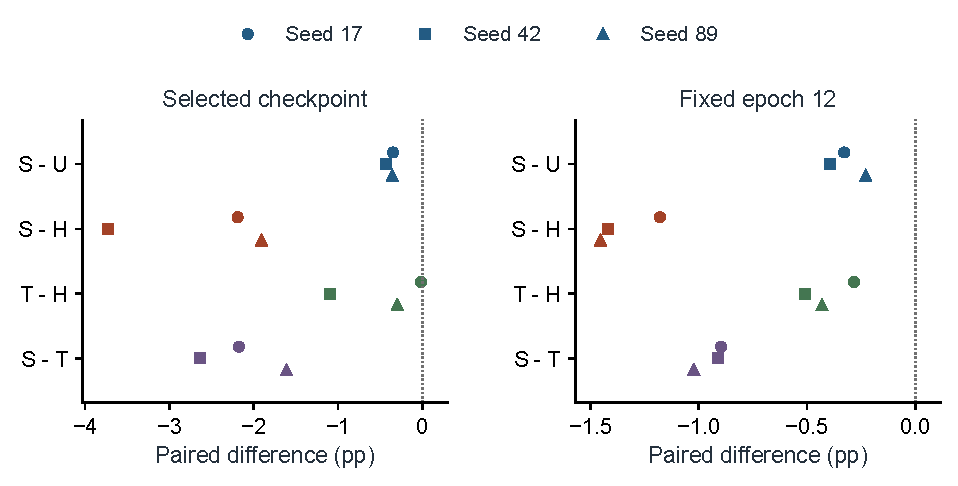
\includegraphics[width=.94\linewidth]{submission_reader_2026_10_13/source/figures/FigS3.pdf}
\caption{Original four conditions: individual paired seed differences at the common-coverage endpoint. (a) Selected and (b) fixed epoch-12 weights. Exact values appear in Table~\ref{tab:seeds}; within-row vertical offsets separate seeds without changing their difference values}
\end{figure}

\begin{figure}[t]
\centering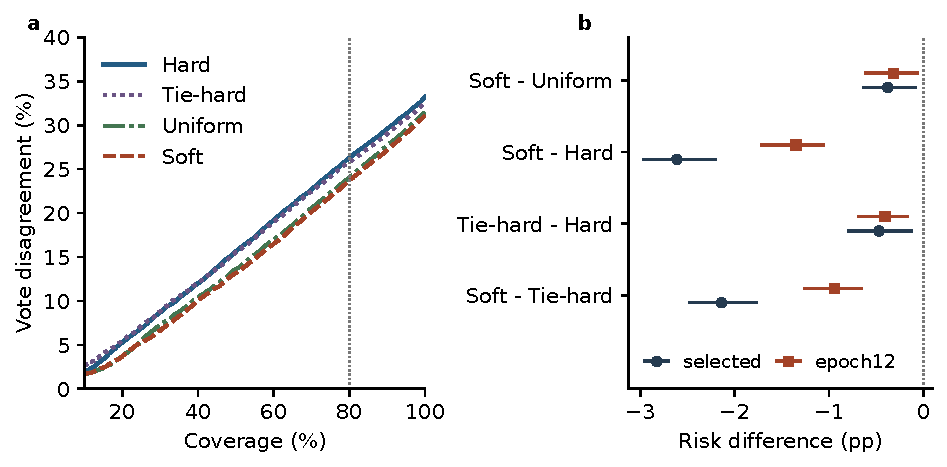
\includegraphics[width=\linewidth]{submission_reader_2026_10_13/source/figures/HistoricalFig2.pdf}
\caption{(a) Original four conditions: mean selected-checkpoint risk--coverage curves across three seeds; the displayed range begins at 10\%, and every prefix is released. (b) Mean paired contrasts and conditional 95\% pixel-cluster intervals, for selected and epoch-12 weights. Negative differences favor the first-named target. Intervals do not measure seed-population or external-domain uncertainty}
\end{figure}

\begin{figure}[ht]\centering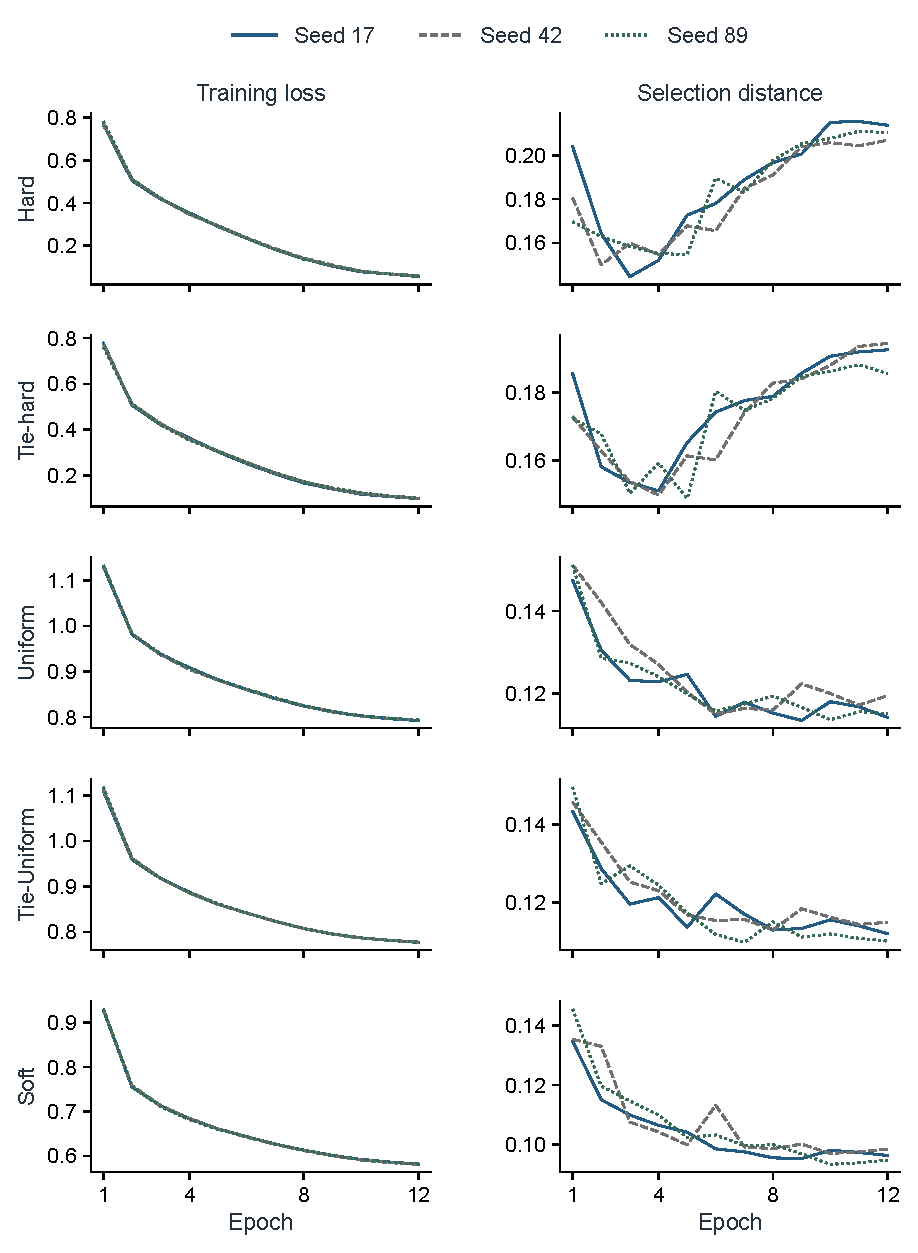
\includegraphics[width=.94\linewidth]{submission_reader_2026_10_13/source/figures/LearningCurves.pdf}\caption{Training loss and selection-distance trajectories for the fifteen retained Swin runs. ResNet trajectories are supplied separately below. The target-dependent loss scales are not comparable performance endpoints.}\end{figure}

\clearpage\section{Distributional agreement and backbone sensitivity}\label{supp:distribution}
The distance is $D=N^{-1}\sum_i\sum_{c=1}^{10}(\tilde p_{ic}-q_{ic})^2$, where $\tilde p$ adds three zeros to the seven outputs. All states use the same $N=3,275$ primary test rows and the original ten-category vote distributions, without renormalization. These descriptive summaries were assembled after the outcomes were known. The measure and per-state values were already recorded. No images are rejected by confidence, and no training or probability ensemble is added.
\begin{table}[H]\caption{Held-out squared distribution distance for every retained target, state and seed. Lower is better; values are distance units, not percentages}\label{tab:distributionseeds}
\centering\small\begin{tabular}{lllrrrr}\toprule
Backbone & State & Target & Seed 17 & Seed 42 & Seed 89 & Mean\\\midrule
Swin-T & Selected & Hard & 0.153453 & 0.157580 & 0.162272 & 0.157769\\
Swin-T & Selected & Tie-hard & 0.163318 & 0.170017 & 0.151180 & 0.161505\\
Swin-T & Selected & Uniform & 0.115093 & 0.115385 & 0.116645 & 0.115708\\
Swin-T & Selected & Tie-Uniform & 0.114356 & 0.116172 & 0.110653 & 0.113727\\
Swin-T & Selected & Soft & 0.098510 & 0.097502 & 0.097491 & 0.097835\\
\addlinespace
Swin-T & Epoch 12 & Hard & 0.226550 & 0.225623 & 0.225190 & 0.225787\\
Swin-T & Epoch 12 & Tie-hard & 0.209374 & 0.205987 & 0.202012 & 0.205791\\
Swin-T & Epoch 12 & Uniform & 0.117631 & 0.117785 & 0.115561 & 0.116992\\
Swin-T & Epoch 12 & Tie-Uniform & 0.114356 & 0.112754 & 0.111290 & 0.112800\\
Swin-T & Epoch 12 & Soft & 0.098639 & 0.097274 & 0.097469 & 0.097794\\
\addlinespace
ResNet-18 & Selected & Uniform & 0.121368 & 0.123774 & 0.123949 & 0.123030\\
ResNet-18 & Selected & Tie-Uniform & 0.119359 & 0.118507 & 0.116272 & 0.118046\\
ResNet-18 & Selected & Soft & 0.109512 & 0.112412 & 0.109837 & 0.110587\\
\addlinespace
ResNet-18 & Epoch 12 & Uniform & 0.121749 & 0.122098 & 0.123936 & 0.122595\\
ResNet-18 & Epoch 12 & Tie-Uniform & 0.115945 & 0.118419 & 0.115596 & 0.116653\\
ResNet-18 & Epoch 12 & Soft & 0.110599 & 0.111553 & 0.110533 & 0.110895\\
\addlinespace
\bottomrule\end{tabular}\end{table}
The companion \texttt{distribution\_distance.csv} retains full precision, prediction hashes and exact agreement with the consolidated original ledger. Soft is lower than both controls for each paired seed in both families and states. These overlapping comparisons are not independent replications, and no new confidence interval or calibration claim is attached.


The main article reports differences and conditional intervals for both checkpoint states. The following table adds absolute ResNet risks, and the figures report the retained learning trajectories and coverage comparisons. Accepted counts and fixed-image comparisons appear in Sections S4 and S3, respectively. These secondary checks were designed adaptively, reuse the same images, and do not rank architectures.

\begin{table}[H]
\caption{ResNet-18 complete-vote risk (\%) at 80\% coverage, means across paired seeds}\label{tab:resnetrisk}
\centering\begin{tabular}{lrr}\toprule
Targets & Selected & Epoch 12\\\midrule
Soft & 24.700 & 24.603\\
Uniform & 24.527 & 24.433\\
Tie-Uniform & 24.658 & 24.413\\
\bottomrule\end{tabular}\par
\end{table}

\begin{figure}[ht]\centering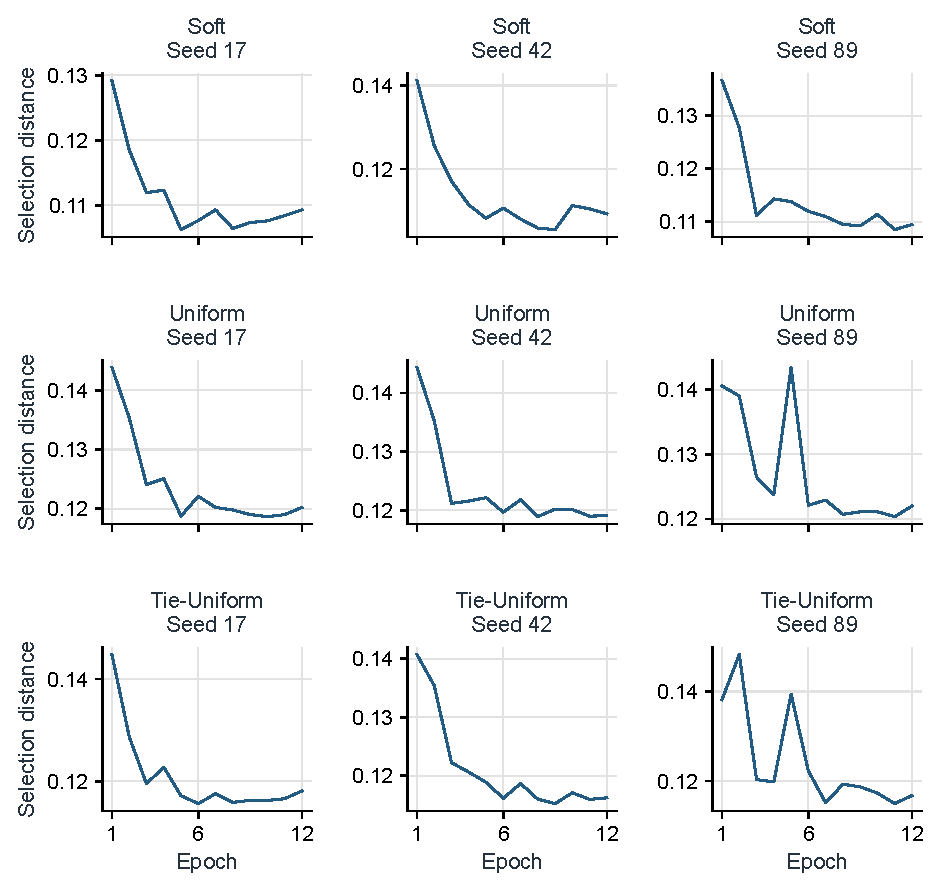
\includegraphics[width=\linewidth]{submission_reader_2026_10_13/source/figures/ResNetLearning.pdf}\caption{Selection-distance trajectories for the nine ResNet runs. Selected and epoch-12 models are both evaluated; these curves do not establish convergence}\end{figure}

\begin{figure}[ht]\centering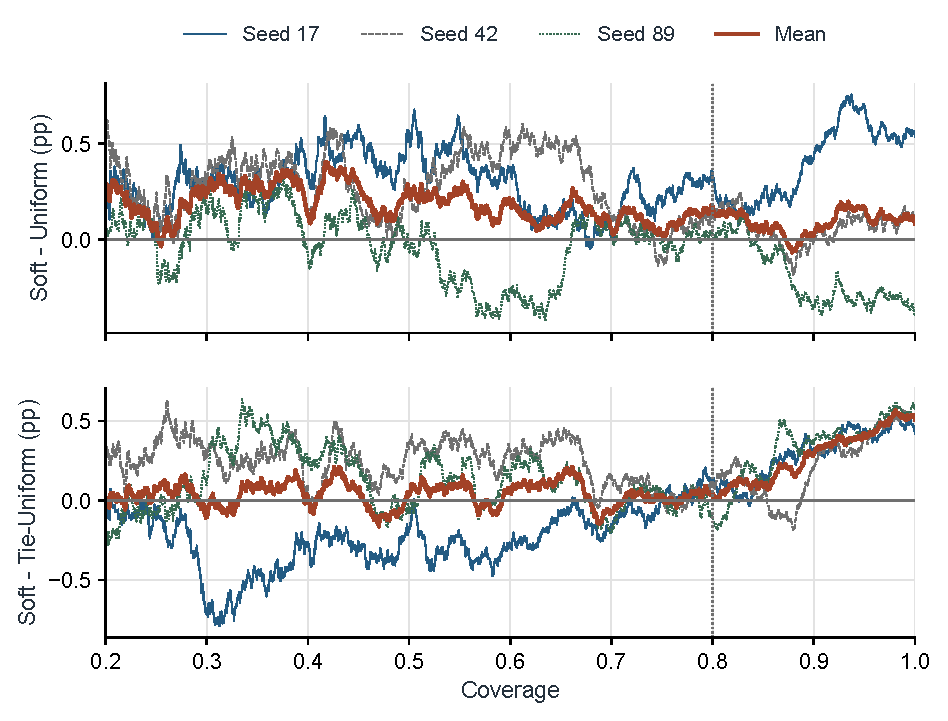
\includegraphics[width=\linewidth]{submission_reader_2026_10_13/source/figures/ResNetDifferences.pdf}\caption{ResNet selected-model own-ranking risk differences at 20--100\% common coverage. Thin curves are paired seeds and thick curves their mean. The dotted marker identifies the prespecified 80\% secondary endpoint. These descriptive curves have no simultaneous uncertainty bands and do not compare predictions on identical accepted images}\end{figure}

\clearpage\section{Accepted-image sets and annotation references}\label{supp:accepted}
\begin{longtable}{llrrr}\caption{Swin-T per-seed fixed-image cross-evaluation}\\\toprule State & Predictor & Seed & Uniform set & Soft set\\\midrule\endhead
selected & Uniform & 17 & 24.0496 & 24.0878\\
selected & Soft & 17 & 24.1145 & 23.7023\\
selected & Uniform & 42 & 24.1718 & 24.1908\\
selected & Soft & 42 & 24.2023 & 23.7405\\
selected & Uniform & 89 & 23.9656 & 23.8321\\
selected & Soft & 89 & 24.1260 & 23.6107\\
epoch12 & Uniform & 17 & 23.9733 & 24.0076\\
epoch12 & Soft & 17 & 23.9389 & 23.6450\\
epoch12 & Uniform & 42 & 24.0840 & 23.8817\\
epoch12 & Soft & 42 & 24.2595 & 23.6908\\
epoch12 & Uniform & 89 & 23.7901 & 23.6489\\
epoch12 & Soft & 89 & 23.9122 & 23.5611\\
\bottomrule\end{longtable}
Risk entries are complete-vote disagreement percentages at exactly 2,620 accepted images.
\begin{longtable}{llrrrr}\caption{Swin-T accepted-set overlap for Soft and Uniform}\\\toprule State & Seed & Intersection & Union & Jaccard & Overlap fraction\\\midrule\endhead
selected & 17 & 2397 & 2843 & 0.8431 & 0.9149\\
selected & 42 & 2381 & 2859 & 0.8328 & 0.9088\\
selected & 89 & 2402 & 2838 & 0.8464 & 0.9168\\
epoch12 & 17 & 2394 & 2846 & 0.8412 & 0.9137\\
epoch12 & 42 & 2391 & 2849 & 0.8392 & 0.9126\\
epoch12 & 89 & 2404 & 2836 & 0.8477 & 0.9176\\
\bottomrule\end{longtable}
Overlap fraction divides the intersection by 2,620, whereas Jaccard divides by the union. The two accepted sets can share most images while their differing tails change mean risk.

\subsection*{Selected-checkpoint fixed-image comparisons}\begin{longtable}{lllrrr}\caption{ResNet-18 selected fixed-image cross-evaluation}\\\toprule Control & Predictor & Selector & Seed 17 & Seed 42 & Seed 89\\\midrule\endhead
Uniform & Soft & Soft & 24.8321 & 24.7824 & 24.4847\\
Uniform & Soft & Uniform & 25.1183 & 25.0382 & 24.7595\\
Uniform & Uniform & Soft & 25.2214 & 25.0687 & 25.0458\\
Uniform & Uniform & Uniform & 24.4847 & 24.6450 & 24.4504\\
Tie-Uniform & Soft & Soft & 24.8321 & 24.7824 & 24.4847\\
Tie-Uniform & Soft & Tie-Uniform & 25.3588 & 25.3397 & 25.1145\\
Tie-Uniform & Tie-Uniform & Soft & 24.9656 & 24.7748 & 24.4313\\
Tie-Uniform & Tie-Uniform & Tie-Uniform & 24.7137 & 24.6679 & 24.5916\\
\bottomrule\end{longtable}
Entries are complete-vote disagreement percentages at 2,620 retained images.

\clearpage
\subsection*{Fixed-epoch fixed-image comparisons}\begin{longtable}{lllrrr}\caption{ResNet-18 epoch 12 fixed-image cross-evaluation}\\\toprule Control & Predictor & Selector & Seed 17 & Seed 42 & Seed 89\\\midrule\endhead
Uniform & Soft & Soft & 24.6069 & 24.6450 & 24.5573\\
Uniform & Soft & Uniform & 24.8702 & 24.7519 & 24.9313\\
Uniform & Uniform & Soft & 24.9275 & 24.8053 & 24.9847\\
Uniform & Uniform & Uniform & 24.5344 & 24.1565 & 24.6069\\
Tie-Uniform & Soft & Soft & 24.6069 & 24.6450 & 24.5573\\
Tie-Uniform & Soft & Tie-Uniform & 24.7176 & 24.9618 & 24.9504\\
Tie-Uniform & Tie-Uniform & Soft & 24.6412 & 24.8779 & 24.6756\\
Tie-Uniform & Tie-Uniform & Tie-Uniform & 24.2824 & 24.5267 & 24.4313\\
\bottomrule\end{longtable}
Entries are complete-vote disagreement percentages at 2,620 retained images.

\begin{longtable}{llrrr}\caption{ResNet-18 reference-specific weighted F1}\\\toprule State & Targets & Original/all & Original/subset & Crowd/subset\\\midrule\endhead
selected & Soft & 0.5564 & 0.6508 & 0.9053\\
selected & Uniform & 0.5558 & 0.6531 & 0.9093\\
selected & Tie-Uniform & 0.5588 & 0.6572 & 0.9181\\
epoch12 & Soft & 0.5612 & 0.6561 & 0.9110\\
epoch12 & Uniform & 0.5563 & 0.6542 & 0.9135\\
epoch12 & Tie-Uniform & 0.5608 & 0.6597 & 0.9209\\
\bottomrule\end{longtable}
All images: 3,275; identical majority subset in the last two columns: 2,484. No extra relabeling is performed. Per-seed unsupported masses and overlaps are supplied in the CSV ledger.

\begin{figure}[ht]\centering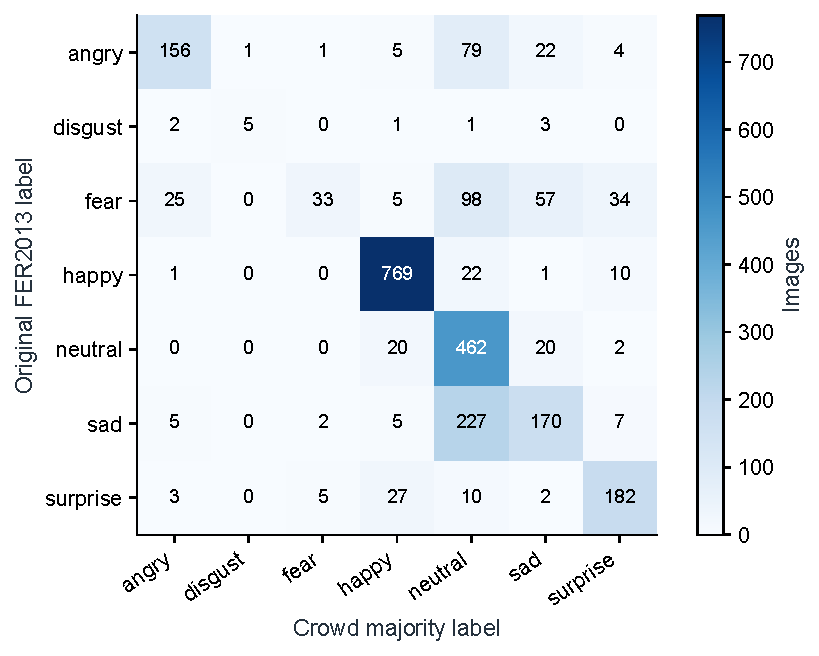
\includegraphics[width=.94\linewidth]{submission_reader_2026_10_13/source/figures/ReferenceConfusion.pdf}\caption{Original-label versus supported crowd-majority reference counts on exactly the same 2,484 primary-test images. This matrix compares references, not predictions.}\end{figure}

\clearpage\section{Effects of unsupported annotation categories}\label{supp:unsupported}
\begin{longtable}{lllrrrr}
\caption{Original four conditions, supported-mass strata: means over three selected-checkpoint seeds. Risk columns are percentages; accepted count can vary by seed}\\
\toprule Targets & Stratum & Selection & N & Accepted & Risk & Supported-only\\\midrule\endfirsthead
\toprule Targets & Stratum & Selection & N & Accepted & Risk & Supported-only\\\midrule\endhead
Hard & full & all & 1732 & 1732.00 & 19.93 & 19.93\\
Hard & full & global80 & 1732 & 1497.33 & 14.96 & 14.96\\
Hard & full & within80 & 1732 & 1386.00 & 12.80 & 12.80\\
Hard & partial & all & 1527 & 1527.00 & 47.53 & 38.44\\
Hard & partial & global80 & 1527 & 1116.33 & 41.08 & 31.30\\
Hard & partial & within80 & 1527 & 1222.00 & 42.69 & 33.04\\
Hard & zero & all & 16 & 16.00 & 100.00 & --\\
Hard & zero & global80 & 16 & 6.33 & 100.00 & --\\
Hard & zero & within80 & 16 & 13.00 & 100.00 & --\\
\addlinespace
Tie-hard & full & all & 1732 & 1732.00 & 19.42 & 19.42\\
Tie-hard & full & global80 & 1732 & 1507.00 & 14.51 & 14.51\\
Tie-hard & full & within80 & 1732 & 1386.00 & 12.33 & 12.33\\
Tie-hard & partial & all & 1527 & 1527.00 & 46.84 & 37.52\\
Tie-hard & partial & global80 & 1527 & 1105.67 & 40.76 & 30.74\\
Tie-hard & partial & within80 & 1527 & 1222.00 & 42.23 & 32.38\\
Tie-hard & zero & all & 16 & 16.00 & 100.00 & --\\
Tie-hard & zero & global80 & 16 & 7.33 & 100.00 & --\\
Tie-hard & zero & within80 & 16 & 13.00 & 100.00 & --\\
\addlinespace
Uniform & full & all & 1732 & 1732.00 & 18.32 & 18.32\\
Uniform & full & global80 & 1732 & 1523.00 & 13.45 & 13.45\\
Uniform & full & within80 & 1732 & 1386.00 & 10.94 & 10.94\\
Uniform & partial & all & 1527 & 1527.00 & 45.71 & 36.24\\
Uniform & partial & global80 & 1527 & 1090.00 & 38.40 & 28.24\\
Uniform & partial & within80 & 1527 & 1222.00 & 40.58 & 30.62\\
Uniform & zero & all & 16 & 16.00 & 100.00 & --\\
Uniform & zero & global80 & 16 & 7.00 & 100.00 & --\\
Uniform & zero & within80 & 16 & 13.00 & 100.00 & --\\
\addlinespace
Soft & full & all & 1732 & 1732.00 & 17.93 & 17.93\\
Soft & full & global80 & 1732 & 1529.00 & 13.23 & 13.23\\
Soft & full & within80 & 1732 & 1386.00 & 10.42 & 10.42\\
Soft & partial & all & 1527 & 1527.00 & 45.36 & 35.75\\
Soft & partial & global80 & 1527 & 1080.00 & 37.71 & 27.35\\
Soft & partial & within80 & 1527 & 1222.00 & 40.00 & 29.77\\
Soft & zero & all & 16 & 16.00 & 100.00 & --\\
Soft & zero & global80 & 16 & 11.00 & 100.00 & --\\
Soft & zero & within80 & 16 & 13.00 & 100.00 & --\\
\addlinespace
\bottomrule\end{longtable}
Full means that all votes fall in the output categories; partial means that some do and some do not; zero means that none do. Risk is necessarily one in the zero stratum because the model cannot predict any category that received a vote. Global selection may leave a stratum empty; its risk is then undefined.

\clearpage
\begin{longtable}{lllrrr}\caption{Unsupported category vote mass by population and accepted-set scope}\\\toprule Targets & Population & Scope & Contempt & Unknown & Not-a-face\\\midrule\endhead
Hard & calibration & all & 1.797 & 3.666 & 0.262\\
Hard & calibration & global80 & 1.525 & 3.092 & 0.185\\
Hard & test & all & 1.554 & 5.667 & 0.656\\
Hard & test & global80 & 1.291 & 4.966 & 0.391\\
Tie-hard & calibration & all & 1.797 & 3.666 & 0.262\\
Tie-hard & calibration & global80 & 1.446 & 3.064 & 0.274\\
Tie-hard & test & all & 1.554 & 5.667 & 0.656\\
Tie-hard & test & global80 & 1.302 & 4.931 & 0.433\\
Uniform & calibration & all & 1.797 & 3.666 & 0.262\\
Uniform & calibration & global80 & 1.329 & 2.877 & 0.193\\
Uniform & test & all & 1.554 & 5.667 & 0.656\\
Uniform & test & global80 & 1.224 & 4.765 & 0.421\\
Tie-Uniform & calibration & all & 1.797 & 3.666 & 0.262\\
Tie-Uniform & calibration & global80 & 1.314 & 2.943 & 0.238\\
Tie-Uniform & test & all & 1.554 & 5.667 & 0.656\\
Tie-Uniform & test & global80 & 1.246 & 4.821 & 0.405\\
Soft & calibration & all & 1.797 & 3.666 & 0.262\\
Soft & calibration & global80 & 1.291 & 3.004 & 0.241\\
Soft & test & all & 1.554 & 5.667 & 0.656\\
Soft & test & global80 & 1.228 & 4.749 & 0.571\\
\bottomrule\end{longtable}
Entries are mean vote-mass percentages across three seeds, not proportions of images with that label. All-image masses are model-independent; global80 conditions on each model's ranking. The three categories do not share one semantic interpretation.

\begin{table}[H]
\caption{ResNet-18 global 80\% accepted counts in full/partial/zero-supported-mass strata. Entries list seeds 17, 42, 89}\label{tab:resnetretention}
\centering\begin{tabular}{lrrr}\toprule
Targets & Full & Partial & Zero\\\midrule
Soft & 1509, 1533, 1522 & 1106, 1077, 1088 & 5, 10, 10\\
Uniform & 1520, 1528, 1522 & 1091, 1085, 1092 & 9, 7, 6\\
Tie-Uniform & 1523, 1521, 1511 & 1088, 1090, 1101 & 9, 9, 8\\
\bottomrule\end{tabular}\par
\smallskip
Each seed retains 2,620 of 3,275 test images. Zero-mass population size is 16.\par
\end{table}

\clearpage\section{Sensitivity to confidence scores}\label{supp:scores}
This additional analysis uses already exposed test predictions. All 24 fitted models and 48 inference states are retained. Probability-only scores never use test votes to rank images. The complete new ledgers cover 20\%, 50\%, 80\% and 100\%; the table below reports 80\%, with 2,620 retained images per model. Seed variation is descriptive, not a confidence interval. No test-selected score or threshold is deployed.
\begin{longtable}{llllrrr}
\caption{All paired seed differences for score sensitivity at 80\% coverage (pp)}\label{tab:scoreseeds}\\
\toprule Backbone & State & Score & Control & Seed 17 & Seed 42 & Seed 89\\\midrule\endfirsthead
\toprule Backbone & State & Score & Control & Seed 17 & Seed 42 & Seed 89\\\midrule\endhead
Swin-T & Selected & MSP & Uniform & -0.3473 & -0.4313 & -0.3550\\
Swin-T & Selected & MSP & Tie-Uniform & -0.3779 & -0.5840 & -0.8015\\
Swin-T & Selected & Margin & Uniform & +0.0534 & -0.3015 & -0.2099\\
Swin-T & Selected & Margin & Tie-Uniform & +0.1412 & -0.3092 & -0.7290\\
Swin-T & Selected & Neg. entropy & Uniform & +0.0267 & -0.1641 & -0.1412\\
Swin-T & Selected & Neg. entropy & Tie-Uniform & -0.1336 & -0.3321 & -0.5038\\
Swin-T & Epoch 12 & MSP & Uniform & -0.3282 & -0.3931 & -0.2290\\
Swin-T & Epoch 12 & MSP & Tie-Uniform & -0.4351 & -0.2214 & -0.2634\\
Swin-T & Epoch 12 & Margin & Uniform & -0.1718 & -0.2977 & +0.1031\\
Swin-T & Epoch 12 & Margin & Tie-Uniform & -0.1794 & -0.1145 & +0.1221\\
Swin-T & Epoch 12 & Neg. entropy & Uniform & -0.1679 & -0.4618 & -0.2595\\
Swin-T & Epoch 12 & Neg. entropy & Tie-Uniform & -0.3168 & -0.1679 & -0.2405\\
ResNet-18 & Selected & MSP & Uniform & +0.3473 & +0.1374 & +0.0344\\
ResNet-18 & Selected & MSP & Tie-Uniform & +0.1183 & +0.1145 & -0.1069\\
ResNet-18 & Selected & Margin & Uniform & +0.6221 & +0.2519 & +0.3779\\
ResNet-18 & Selected & Margin & Tie-Uniform & +0.2519 & +0.2099 & +0.1565\\
ResNet-18 & Selected & Neg. entropy & Uniform & +0.6069 & +0.5840 & +0.3359\\
ResNet-18 & Selected & Neg. entropy & Tie-Uniform & +0.4656 & +0.5229 & +0.4656\\
ResNet-18 & Epoch 12 & MSP & Uniform & +0.0725 & +0.4885 & -0.0496\\
ResNet-18 & Epoch 12 & MSP & Tie-Uniform & +0.3244 & +0.1183 & +0.1260\\
ResNet-18 & Epoch 12 & Margin & Uniform & +0.3664 & +0.7863 & +0.3817\\
ResNet-18 & Epoch 12 & Margin & Tie-Uniform & +0.6145 & +0.6260 & +0.4237\\
ResNet-18 & Epoch 12 & Neg. entropy & Uniform & +0.2595 & +0.5076 & +0.1527\\
ResNet-18 & Epoch 12 & Neg. entropy & Tie-Uniform & +0.4580 & +0.2595 & +0.5878\\
\bottomrule\end{longtable}
\clearpage\begin{figure}[H]\centering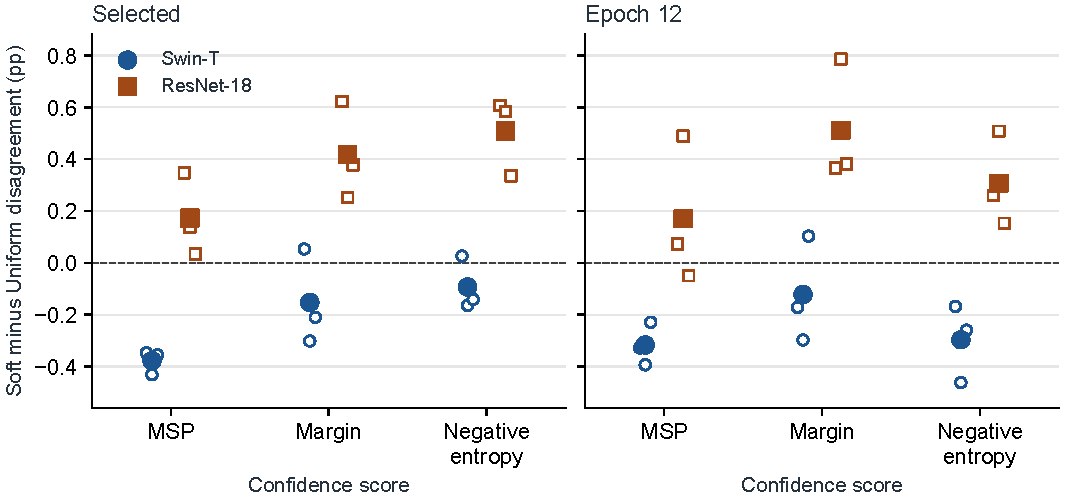
\includegraphics[width=\linewidth]{submission_reader_2026_10_13/source/figures/SelectorSensitivity.pdf}
\caption{Probability-only score sensitivity at 80\% own-ranking coverage for Soft minus Uniform. (a) Selected checkpoints; (b) fixed epoch 12. Small hollow symbols are the three paired seeds, horizontally offset only for visibility; large filled symbols are their mean. All panels share a vertical scale. Negative values favor Soft. There are no uncertainty bars; seed dispersion is not population uncertainty. The categorical score choices are not an ordered tuning path. Some Swin seed differences cross zero; no score was selected after observing these outcomes}\label{fig:scores}\end{figure}

\clearpage\section{Calibration-to-test transfer}\label{supp:calibration}
\begin{longtable}{llrrrr}
\caption{Original four conditions, calibration half-split holdout-minus-fit risk gaps. Means and 5th/95th percentiles are descriptive percentage points over nonempty seed--split outcomes, not confidence intervals}\\
\toprule Supervision & Risk target & Nonempty & Mean gap & 5th pct. & 95th pct.\\\midrule\endfirsthead
\toprule Supervision & Risk target & Nonempty & Mean gap & 5th pct. & 95th pct.\\\midrule\endhead
Hard & 10\% & 300/300 & -0.040 & -2.215 & +2.175\\
Hard & 20\% & 300/300 & +0.050 & -2.328 & +2.590\\
Hard & 30\% & 300/300 & +0.008 & -2.752 & +2.598\\
Tie-hard & 10\% & 300/300 & -0.002 & -2.169 & +2.399\\
Tie-hard & 20\% & 300/300 & +0.180 & -2.344 & +2.770\\
Tie-hard & 30\% & 300/300 & +0.072 & -2.683 & +2.859\\
Uniform & 10\% & 300/300 & +0.216 & -1.808 & +2.033\\
Uniform & 20\% & 300/300 & +0.193 & -2.021 & +2.617\\
Uniform & 30\% & 300/300 & +0.037 & -2.442 & +2.536\\
Soft & 10\% & 300/300 & +0.060 & -1.871 & +1.736\\
Soft & 20\% & 300/300 & +0.170 & -2.004 & +2.428\\
Soft & 30\% & 300/300 & +0.015 & -2.410 & +2.736\\
\bottomrule\end{longtable}
Each of 100 shared pixel-cluster splits uses disjoint calibration halves for fitting and checking the empirical threshold. Splits overlap one another. Minimum fitted accepted count is 100 and score ties are never split. The full ledger includes fit/holdout counts, risks, thresholds, and holdout coverage for every split, including empty policies.

Calibration: unsupported mass 5.7247\%, supported ambiguity 17.9720\%, annotation floor 23.6967\%.\par
Test: unsupported mass 7.8779\%, supported ambiguity 18.7878\%, annotation floor 26.6656\%.\par
These quantities use annotations only and do not depend on the fitted model. The main figure instead reports differences on the images accepted by each model's threshold. Those differences can depart from the full-population values. Neither comparison identifies a unique cause of target overshoot.

\clearpage\section{External clip evaluation and diagnostic analyses}\label{supp:external}
The external unit is a video-only speech clip, not an image or frame judgment. All 1,440 clips and 24 actors are retained in the coverage denominator. The protocol, raw-vote adapter, integrity manifests, all frame/clip probabilities and five CSV ledgers are in Online Resource 8. No new training or test-fitted threshold is performed. Raw nine-category responses preserve calm and none; the merged sensitivity adds calm to neutral and leaves none unchanged. Actor intervals are in the main paper; seed dispersion below is descriptive.
\begin{longtable}{lllrrr}
\caption{External frame eligibility by actor}\\
\toprule Actor & Clips & Eligible & Valid frames & Attempted frames & Max. coverage (\%)\\\midrule\endfirsthead
\toprule Actor & Clips & Eligible & Valid frames & Attempted frames & Max. coverage (\%)\\\midrule\endhead
01 & 60 & 60 & 480 & 480 & 100.00\\
02 & 60 & 60 & 480 & 480 & 100.00\\
03 & 60 & 60 & 480 & 480 & 100.00\\
04 & 60 & 60 & 480 & 480 & 100.00\\
05 & 60 & 60 & 480 & 480 & 100.00\\
06 & 60 & 60 & 480 & 480 & 100.00\\
07 & 60 & 60 & 480 & 480 & 100.00\\
08 & 60 & 60 & 480 & 480 & 100.00\\
09 & 60 & 60 & 480 & 480 & 100.00\\
10 & 60 & 60 & 480 & 480 & 100.00\\
11 & 60 & 60 & 480 & 480 & 100.00\\
12 & 60 & 60 & 480 & 480 & 100.00\\
13 & 60 & 60 & 480 & 480 & 100.00\\
14 & 60 & 60 & 480 & 480 & 100.00\\
15 & 60 & 60 & 480 & 480 & 100.00\\
16 & 60 & 60 & 480 & 480 & 100.00\\
17 & 60 & 60 & 480 & 480 & 100.00\\
18 & 60 & 60 & 480 & 480 & 100.00\\
19 & 60 & 60 & 480 & 480 & 100.00\\
20 & 60 & 60 & 480 & 480 & 100.00\\
21 & 60 & 60 & 480 & 480 & 100.00\\
22 & 60 & 60 & 480 & 480 & 100.00\\
23 & 60 & 60 & 480 & 480 & 100.00\\
24 & 60 & 60 & 480 & 480 & 100.00\\
\bottomrule\end{longtable}
\clearpage
\begin{longtable}{lllllrrr}
\caption{External 80\% contrasts for every paired seed (pp)}\\
\toprule Model & State & Ref. & Score & Control & 17 & 42 & 89\\\midrule\endfirsthead
\toprule Model & State & Ref. & Score & Control & 17 & 42 & 89\\\midrule\endhead
Swin-T & Sel. & Raw & MSP & Uniform & -0.052 & +2.639 & -0.755\\
Swin-T & Sel. & Raw & MSP & Tie-Uniform & +1.007 & +2.075 & -0.252\\
Swin-T & Sel. & Raw & Margin & Uniform & +0.773 & +3.481 & -0.920\\
Swin-T & Sel. & Raw & Margin & Tie-Uniform & +1.120 & +2.708 & +0.174\\
Swin-T & Sel. & Raw & Neg. entropy & Uniform & +0.217 & +1.875 & -1.024\\
Swin-T & Sel. & Raw & Neg. entropy & Tie-Uniform & +0.755 & +1.580 & -0.625\\
Swin-T & Sel. & Merged & MSP & Uniform & -1.276 & +2.483 & -0.903\\
Swin-T & Sel. & Merged & MSP & Tie-Uniform & +0.747 & +1.545 & -0.226\\
Swin-T & Sel. & Merged & Margin & Uniform & +0.009 & +3.585 & -0.859\\
Swin-T & Sel. & Merged & Margin & Tie-Uniform & +1.259 & +2.300 & +0.339\\
Swin-T & Sel. & Merged & Neg. entropy & Uniform & -0.825 & +1.641 & -1.146\\
Swin-T & Sel. & Merged & Neg. entropy & Tie-Uniform & +0.807 & +1.267 & -0.625\\
Swin-T & E12 & Raw & MSP & Uniform & -0.460 & +1.024 & +0.113\\
Swin-T & E12 & Raw & MSP & Tie-Uniform & +0.495 & +2.535 & -0.608\\
Swin-T & E12 & Raw & Margin & Uniform & +0.139 & +2.266 & +0.365\\
Swin-T & E12 & Raw & Margin & Tie-Uniform & +0.130 & +3.377 & -0.703\\
Swin-T & E12 & Raw & Neg. entropy & Uniform & -0.799 & +1.250 & -0.122\\
Swin-T & E12 & Raw & Neg. entropy & Tie-Uniform & -0.052 & +2.405 & -0.998\\
Swin-T & E12 & Merged & MSP & Uniform & -1.701 & -0.330 & -0.677\\
Swin-T & E12 & Merged & MSP & Tie-Uniform & +0.226 & +1.155 & -0.434\\
Swin-T & E12 & Merged & Margin & Uniform & -0.677 & +1.137 & -0.139\\
Swin-T & E12 & Merged & Margin & Tie-Uniform & +0.165 & +2.326 & -0.451\\
Swin-T & E12 & Merged & Neg. entropy & Uniform & -1.910 & -0.104 & -0.937\\
Swin-T & E12 & Merged & Neg. entropy & Tie-Uniform & -0.078 & +1.016 & -0.825\\
ResNet-18 & Sel. & Raw & MSP & Uniform & +1.042 & +5.521 & -1.068\\
ResNet-18 & Sel. & Raw & MSP & Tie-Uniform & +0.955 & +4.219 & -2.917\\
ResNet-18 & Sel. & Raw & Margin & Uniform & +1.658 & +6.345 & -0.278\\
ResNet-18 & Sel. & Raw & Margin & Tie-Uniform & +1.806 & +4.193 & -2.118\\
ResNet-18 & Sel. & Raw & Neg. entropy & Uniform & +0.200 & +3.377 & -1.675\\
ResNet-18 & Sel. & Raw & Neg. entropy & Tie-Uniform & +0.486 & +2.856 & -2.387\\
ResNet-18 & Sel. & Merged & MSP & Uniform & +1.111 & +3.776 & -0.911\\
ResNet-18 & Sel. & Merged & MSP & Tie-Uniform & +1.189 & +3.750 & -2.717\\
ResNet-18 & Sel. & Merged & Margin & Uniform & +1.693 & +4.332 & +0.391\\
ResNet-18 & Sel. & Merged & Margin & Tie-Uniform & +2.161 & +3.724 & -1.389\\
ResNet-18 & Sel. & Merged & Neg. entropy & Uniform & +0.434 & +1.510 & -1.293\\
ResNet-18 & Sel. & Merged & Neg. entropy & Tie-Uniform & +0.816 & +2.214 & -1.866\\
ResNet-18 & E12 & Raw & MSP & Uniform & +2.196 & +3.064 & -0.148\\
ResNet-18 & E12 & Raw & MSP & Tie-Uniform & +1.832 & +2.474 & -1.745\\
ResNet-18 & E12 & Raw & Margin & Uniform & +2.318 & +3.776 & +0.339\\
ResNet-18 & E12 & Raw & Margin & Tie-Uniform & +2.691 & +3.238 & -1.094\\
ResNet-18 & E12 & Raw & Neg. entropy & Uniform & +2.335 & +1.701 & -1.059\\
ResNet-18 & E12 & Raw & Neg. entropy & Tie-Uniform & +2.040 & +1.866 & -1.997\\
ResNet-18 & E12 & Merged & MSP & Uniform & +2.274 & +1.806 & -0.234\\
ResNet-18 & E12 & Merged & MSP & Tie-Uniform & +2.144 & +2.283 & -1.771\\
ResNet-18 & E12 & Merged & Margin & Uniform & +3.125 & +2.648 & +0.530\\
ResNet-18 & E12 & Merged & Margin & Tie-Uniform & +3.628 & +3.116 & -0.747\\
ResNet-18 & E12 & Merged & Neg. entropy & Uniform & +2.309 & +0.304 & -1.042\\
ResNet-18 & E12 & Merged & Neg. entropy & Tie-Uniform & +2.075 & +1.389 & -1.753\\
\bottomrule\end{longtable}
\clearpage\begin{figure}[H]\centering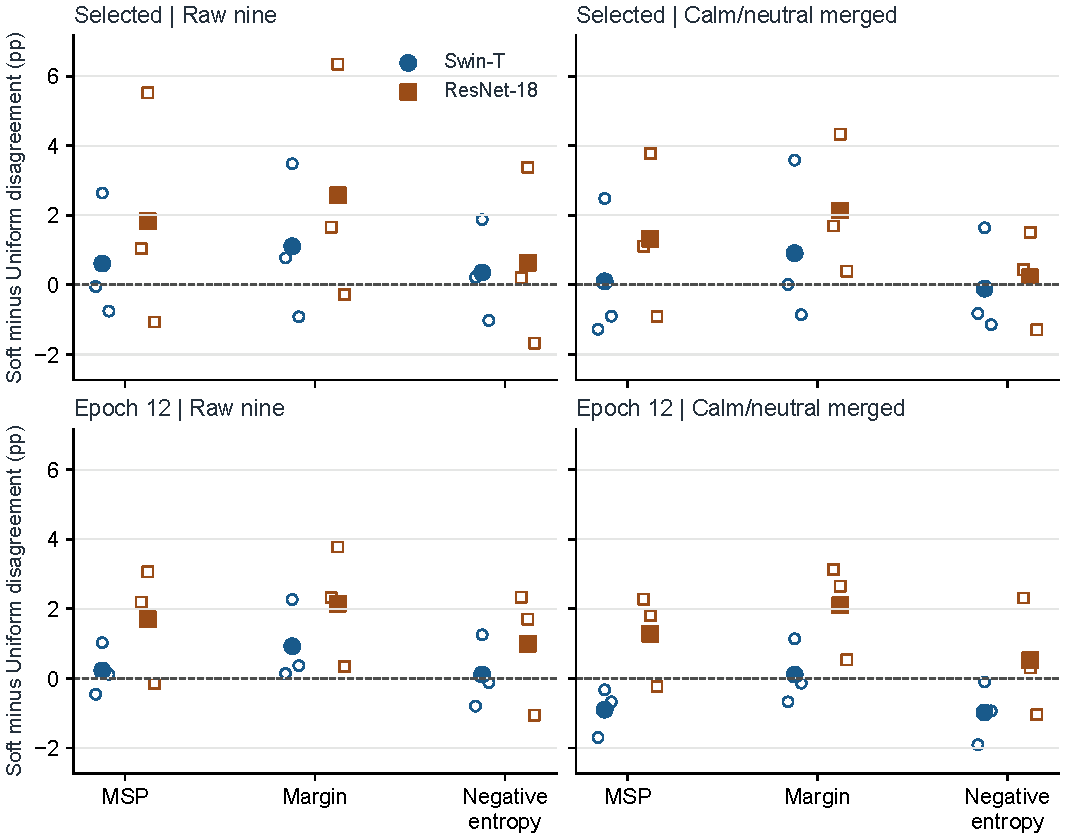
\includegraphics[width=\linewidth]{submission_reader_2026_10_13/source/figures/ExternalScores.pdf}
\caption{External confidence-score sensitivity at 80\% coverage for Soft minus Uniform. Hollow marks are the three paired seeds; filled marks are their means. Panels separate checkpoint state and vote reference. All panels share the same vertical scale. These are own-ranking comparisons, not fixed-image comparisons. Seed dispersion is not an actor interval and no score is selected for deployment from this plot}\end{figure}
\clearpage\begin{longtable}{llllrrrr}
\caption{External 80\% MSP fixed-image cross-evaluation: mean risk across paired seeds (\%)}\\
\toprule Model & State & Ref. & Control & S on S & C on S & S on C & C on C\\\midrule\endfirsthead
\toprule Model & State & Ref. & Control & S on S & C on S & S on C & C on C\\\midrule\endhead
Swin-T & Sel. & Raw & Uniform & 68.37 & 68.22 & 68.07 & 67.75\\
Swin-T & Sel. & Raw & Tie-Uniform & 68.37 & 68.00 & 67.78 & 67.42\\
Swin-T & Sel. & Merged & Uniform & 60.72 & 60.82 & 60.77 & 60.62\\
Swin-T & Sel. & Merged & Tie-Uniform & 60.72 & 60.39 & 60.37 & 60.03\\
Swin-T & E12 & Raw & Uniform & 68.25 & 67.97 & 68.26 & 68.03\\
Swin-T & E12 & Raw & Tie-Uniform & 68.25 & 67.78 & 68.04 & 67.45\\
Swin-T & E12 & Merged & Uniform & 60.47 & 61.03 & 61.08 & 61.37\\
Swin-T & E12 & Merged & Tie-Uniform & 60.47 & 60.34 & 60.47 & 60.16\\
ResNet-18 & Sel. & Raw & Uniform & 71.49 & 70.47 & 70.78 & 69.66\\
ResNet-18 & Sel. & Raw & Tie-Uniform & 71.49 & 70.87 & 71.12 & 70.73\\
ResNet-18 & Sel. & Merged & Uniform & 63.20 & 62.54 & 62.58 & 61.88\\
ResNet-18 & Sel. & Merged & Tie-Uniform & 63.20 & 62.52 & 62.92 & 62.46\\
ResNet-18 & E12 & Raw & Uniform & 71.32 & 70.49 & 70.60 & 69.62\\
ResNet-18 & E12 & Raw & Tie-Uniform & 71.32 & 70.72 & 71.05 & 70.47\\
ResNet-18 & E12 & Merged & Uniform & 63.24 & 62.63 & 62.59 & 61.96\\
ResNet-18 & E12 & Merged & Tie-Uniform & 63.24 & 62.60 & 62.89 & 62.35\\
\bottomrule\end{longtable}
S denotes Soft and C the named control. ``S on C'' applies Soft predictions to the clips accepted by the control. Every available cell uses the same nominal count of 1,152 clips. Per-seed values are retained in the CSV; these cross-evaluations are descriptive, not causal attribution.
\begin{longtable}{lllrrrrr}
\caption{External all-eligible MSP-independent risk accounting: paired-seed means (\%)}\\
\toprule Model & State & Ref. & Risk & Unsupported & Ambiguity & Excess & Coverage\\\midrule\endfirsthead
\toprule Model & State & Ref. & Risk & Unsupported & Ambiguity & Excess & Coverage\\\midrule\endhead
Swin-T S & Sel. & Raw & 71.06 & 11.90 & 16.81 & 42.36 & 100.00\\
Swin-T U & Sel. & Raw & 70.81 & 11.90 & 16.81 & 42.11 & 100.00\\
Swin-T TU & Sel. & Raw & 70.45 & 11.90 & 16.81 & 41.75 & 100.00\\
Swin-T S & Sel. & Merged & 64.84 & 3.14 & 20.23 & 41.47 & 100.00\\
Swin-T U & Sel. & Merged & 64.81 & 3.14 & 20.23 & 41.44 & 100.00\\
Swin-T TU & Sel. & Merged & 64.26 & 3.14 & 20.23 & 40.89 & 100.00\\
Swin-T S & E12 & Raw & 70.95 & 11.90 & 16.81 & 42.25 & 100.00\\
Swin-T U & E12 & Raw & 70.54 & 11.90 & 16.81 & 41.84 & 100.00\\
Swin-T TU & E12 & Raw & 70.62 & 11.90 & 16.81 & 41.92 & 100.00\\
Swin-T S & E12 & Merged & 64.59 & 3.14 & 20.23 & 41.22 & 100.00\\
Swin-T U & E12 & Merged & 64.94 & 3.14 & 20.23 & 41.57 & 100.00\\
Swin-T TU & E12 & Merged & 64.51 & 3.14 & 20.23 & 41.15 & 100.00\\
ResNet-18 S & Sel. & Raw & 74.41 & 11.90 & 16.81 & 45.71 & 100.00\\
ResNet-18 U & Sel. & Raw & 72.87 & 11.90 & 16.81 & 44.16 & 100.00\\
ResNet-18 TU & Sel. & Raw & 73.41 & 11.90 & 16.81 & 44.70 & 100.00\\
ResNet-18 S & Sel. & Merged & 67.62 & 3.14 & 20.23 & 44.25 & 100.00\\
ResNet-18 U & Sel. & Merged & 66.44 & 3.14 & 20.23 & 43.07 & 100.00\\
ResNet-18 TU & Sel. & Merged & 66.58 & 3.14 & 20.23 & 43.21 & 100.00\\
ResNet-18 S & E12 & Raw & 74.69 & 11.90 & 16.81 & 45.99 & 100.00\\
ResNet-18 U & E12 & Raw & 72.58 & 11.90 & 16.81 & 43.87 & 100.00\\
ResNet-18 TU & E12 & Raw & 73.05 & 11.90 & 16.81 & 44.35 & 100.00\\
ResNet-18 S & E12 & Merged & 67.97 & 3.14 & 20.23 & 44.60 & 100.00\\
ResNet-18 U & E12 & Merged & 66.18 & 3.14 & 20.23 & 42.81 & 100.00\\
ResNet-18 TU & E12 & Merged & 66.37 & 3.14 & 20.23 & 43.00 & 100.00\\
\bottomrule\end{longtable}
All-eligible is not relabeled 100\% when a clip fails. Risk equals unsupported plus supported ambiguity plus excess before rounding. U denotes Uniform, TU Tie-Uniform. Raw/merged values score unchanged predictions; the accepted population and all-eligible coverage do not change with reference.

\clearpage\section*{Post hoc external output diagnostics}

The 12 October 2026 addendum was written before these computations, but after the external outcomes were known. No fitting, peak selection or new inferential test was performed. Exports include all 36 frozen states and both populations. The displays below show all three selected Swin Soft/Uniform seeds, not only favorable ones.

\begin{table}[H]
\caption{Principal selected Swin predicted-category proportions at 80\% MSP (\%). Columns retain every seed; each contains 1,152 clips}\label{tab:externalcategories}
\centering\small\begin{tabular}{lrrrrrr}\toprule
 & \multicolumn{3}{c}{Soft} & \multicolumn{3}{c}{Uniform}\\
Category & 17 & 42 & 89 & 17 & 42 & 89\\\midrule
Angry & 0.87 & 1.13 & 1.22 & 1.48 & 1.74 & 1.22\\
Disgust & 0.35 & 0.00 & 0.09 & 0.61 & 0.17 & 0.00\\
Fear & 0.00 & 0.00 & 0.00 & 0.00 & 0.00 & 0.00\\
Happy & 23.96 & 23.18 & 23.70 & 26.74 & 24.57 & 22.92\\
Neutral & 68.14 & 69.97 & 67.01 & 64.58 & 62.67 & 68.32\\
Sad & 3.04 & 2.78 & 3.65 & 3.04 & 5.56 & 3.30\\
Surprise & 3.65 & 2.95 & 4.34 & 3.56 & 5.30 & 4.25\\
\bottomrule\end{tabular}\end{table}

Across all 1,440 clips, raw human-vote mass (\%) is angry: 14.46, disgust: 11.66, fear: 11.21, happy: 16.77, neutral: 9.06, sad: 14.21, surprise: 10.74, calm: 8.76, none: 3.14. Accepted-set vote masses are exported separately for every state and seed; model counts and reference vote mass are distinct quantities.

\begin{figure}[H]\centering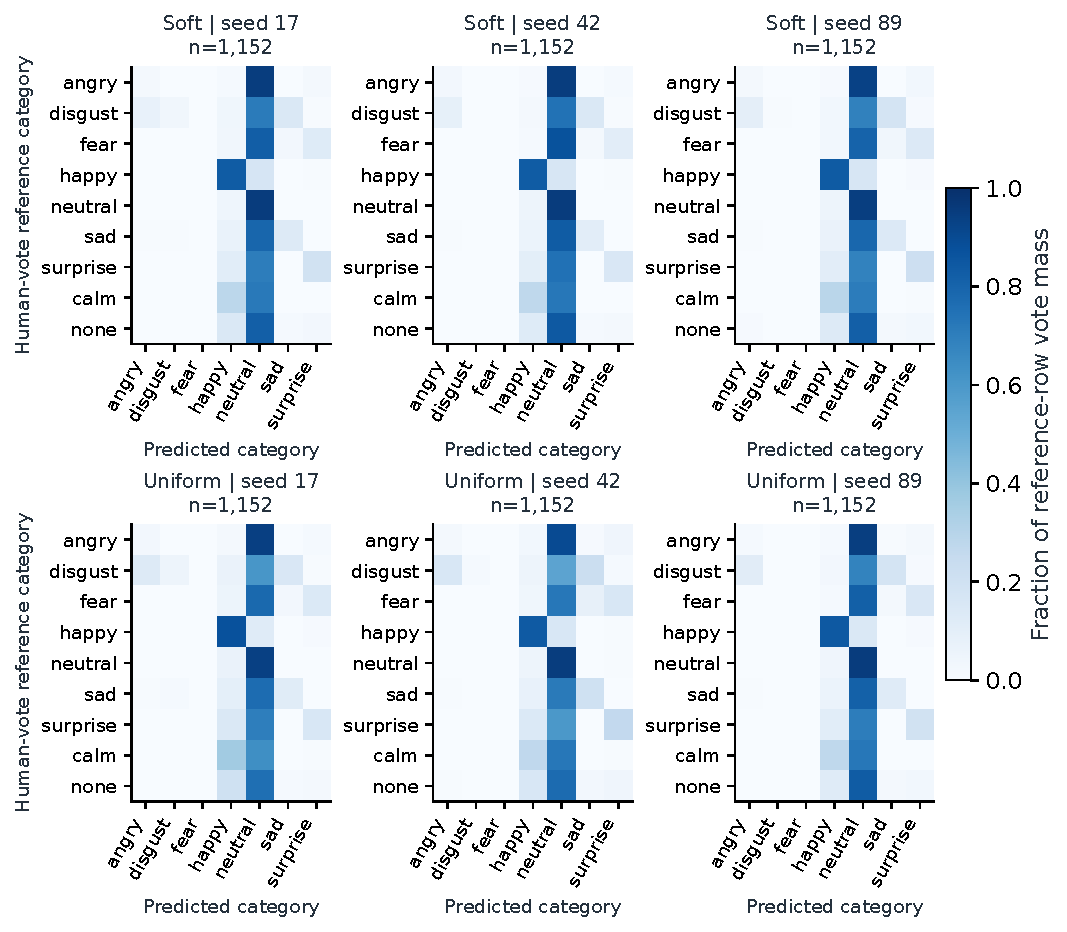
\includegraphics[width=\linewidth]{submission_reader_2026_10_13/source/figures/ExternalVoteMatrices.pdf}

\caption{Human-vote reference versus predicted category for all principal selected Swin Soft/Uniform seeds at 80\% MSP. Each cell divides the vote mass assigned to that predicted column by the row total; it is not single-label confusion or frame accuracy. Calm and none rows remain although the model has no corresponding outputs. Every panel contains 1,152 clips. All 36 states, both populations, raw contributions, row masses and both references are in Online Resource 8. Rows with no vote mass are undefined, not zero. The common scale is 0--1}\end{figure}

\clearpage\begin{figure}[H]\centering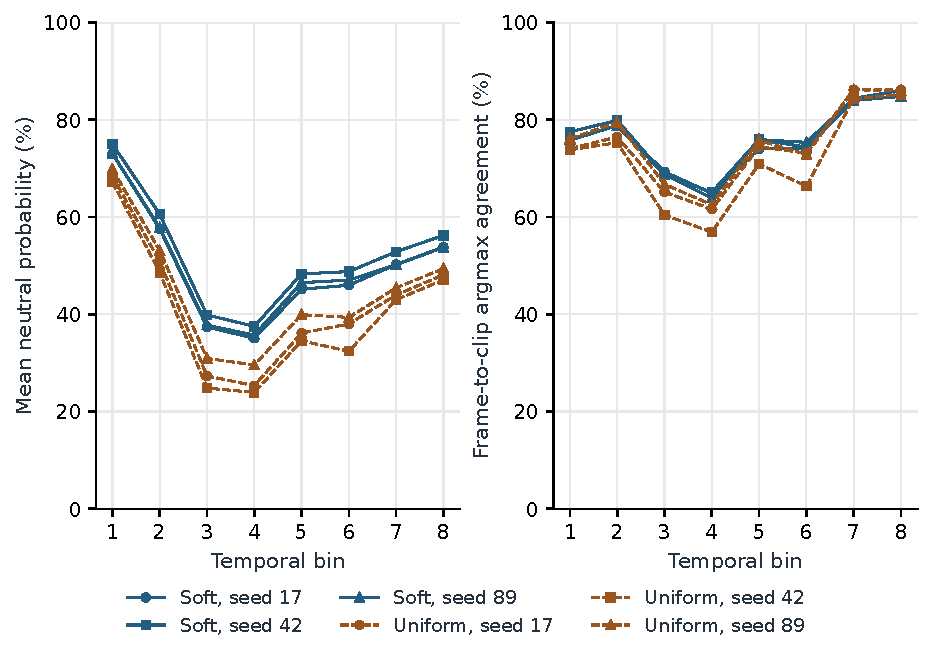
\includegraphics[width=\linewidth]{submission_reader_2026_10_13/source/figures/ExternalTemporal.pdf}

\caption{Predictions across all eight temporal bins for selected Swin Soft/Uniform and all three seeds. Left: mean neutral probability. Right: agreement between frame-level and mean-probability clip predictions from the same model. Each bin has 1,440 valid frames from 1,440 clips; each state has 11,520 frames. Human judgments are clip-level, so agreement is not frame accuracy. Exports include all categories and all 36 states. Temporal patterns do not establish why external disagreement occurs}\end{figure}

Acquisition checks verify video-only speech IDs, ten responses per clip, primary response mapping, frame-bin indices, shared crop validity and canonical category order. Every clip has eight valid frames. Independently summing retained float32 frame probabilities in float64 reproduces the clip mean exactly (maximum absolute difference zero). Raw/merged scoring preserves predictions and accepted IDs. Diagnostic identities use tolerance $10^{-10}$ for vote-mass summation and $10^{-14}$ for clip aggregation; probability normalization tolerance is $10^{-6}$.


\clearpage\section{Model and prototype implementation}\label{supp:implementation}
\begin{figure}[ht]
\centering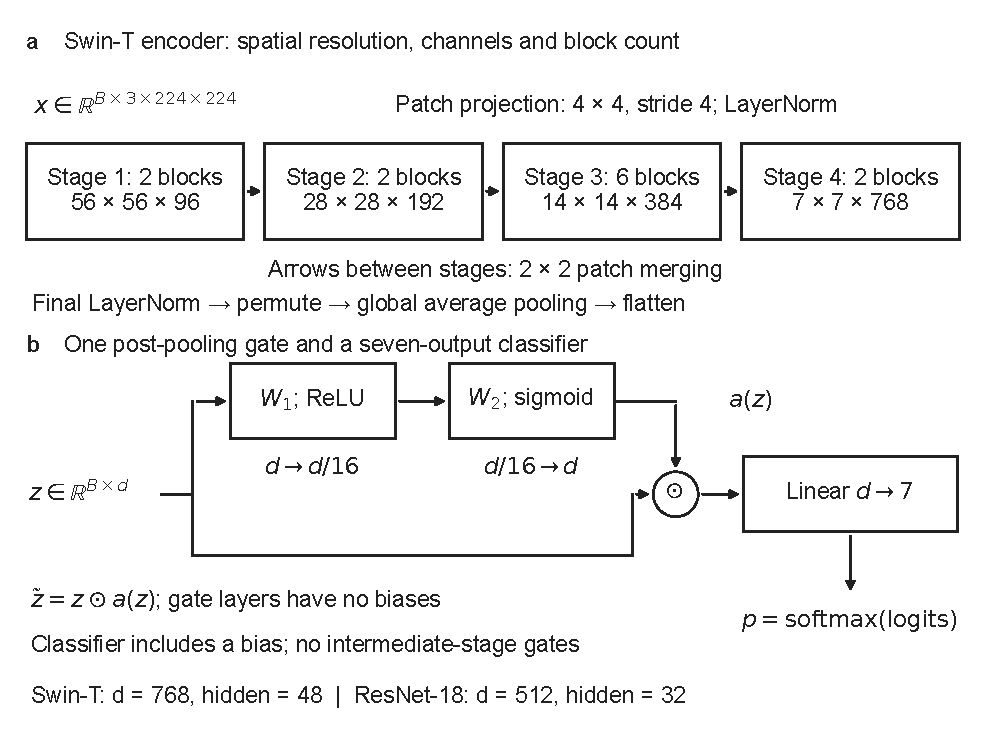
\includegraphics[width=\linewidth]{submission_reader_2026_10_13/source/figures/Fig2.pdf}
\caption{Consolidated implementation diagram, not an architectural contribution. (a) Swin-T hierarchy; stage labels are $H\times W\times C$. (b) One bias-free $768\to48\to768$ ReLU/sigmoid gate acts on the pooled vector through an unchanged bypass and elementwise product, followed by a biased seven-logit classifier. ResNet-18 replaces the encoder and uses a $512\to32\to512$ gate. Architecture is fixed within a backbone; no stage-wise or temporal gate is used}
\end{figure}

\begin{figure}[ht]
\centering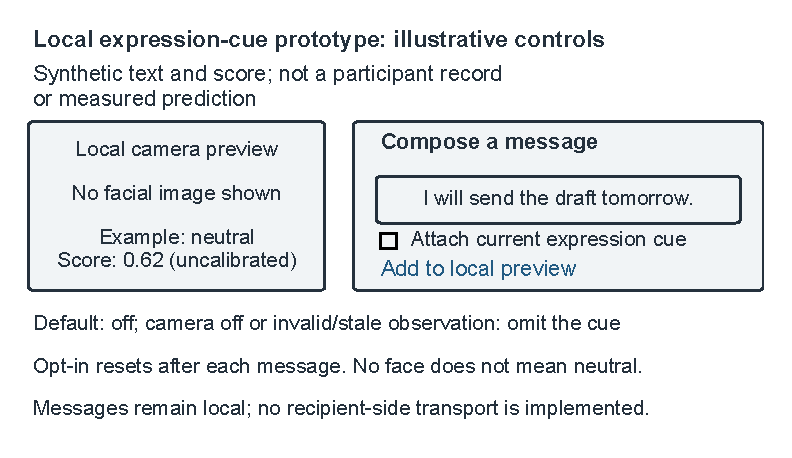
\includegraphics[width=.88\linewidth]{submission_reader_2026_10_13/source/figures/FigS2.pdf}
\caption{Synthetic illustration of the local sender-controlled interface. Text and category presentation are illustrative, not participant observations or a measured prediction. No recipient transport is implemented}
\end{figure}

Online Resource 1 supplies the implementation code; this section provides a dimensioned model diagram (Fig.~S11) and a synthetic interface illustration (Fig.~S12). The latter is not a participant observation or a measured prediction.
The application uses MediaPipe Face Detection with model selection 1 and minimum detection confidence 0.5 (MediaPipe Face Detection; main reference list). Exactly one detected face with a valid clipped crop is eligible. The crop then uses the same grayscale, resize, normalization, class order, and model head as the experiment. Benchmark images are already cropped and do not pass through the detector. Offline predictions use the recorded BF16 evaluation path; the application uses its documented FP32 inference path, so bitwise equality across paths is not assumed.

Predictions are requested no more often than once per second. A category can accompany a message only if the sender opts in, the camera is active, and a valid observation is at most 2.5 seconds old. Attachment is off by default and resets after submission. The cue is withheld when no face or multiple faces are detected, when an observation is stale, or when processing fails. These cases are not labeled neutral. The choices have not been empirically optimized. The interface labels its top-class score as uncalibrated. The confidence policies studied in the paper remain offline; they are not proven runtime protections.

Processing is local only when the Streamlit/Python backend runs on the sender's machine. The supplied configuration uses loopback, disables usage statistics and omits external ICE servers. The application processes frames in memory and does not intentionally record them. Messages stay in session memory for local preview; the application does not send them to a recipient. The category cue can itself be sensitive. These design choices are not a formal privacy guarantee and do not rule out behavior by the operating system or dependencies.

Code and numerical checks cover checkpoint metadata, gating placement, preprocessing, deterministic splits and augmentation, weighted losses, score ties, empty selections, metric definitions, and cue failure states. Runtime checks are software diagnostics, not a naturalistic usability study.

\clearpage\section{Execution provenance and reproduction}\label{supp:provenance}
The execution records below document data handling and the timing of analysis decisions. They supplement the scientific procedures in the main Methods; they do not alter the adaptive or exploratory status of any comparison.

\subsection*{FER2013 acquisition and FER+ alignment}
We acquired the CSV on 20 September 2026 from Kaggle mirror \texttt{deadskull7/fer2013}, version 1, not from an official maintainer distribution. The join follows the official FER+ conversion script's row indexing, not its output filenames, which can be blank or duplicated. A separate raw-source audit checks all 35,887 original emotion IDs, pixel byte hashes and partition positions against the retained manifest. We reorder named vote columns to the fixed model class order. Online Resource 1 contains acquisition and split manifests, the original annotation records, the row adapter and the raw-source audit.

\subsection*{External protocol and integrity records}
We froze the local protocol on 11 October 2026 at 18:17:50 UTC, before computing external model outcomes. It records implementation, annotation, detector and checkpoint hashes. Internal outcomes and external annotation summaries were already known. The pre-outcome amendment corrects the disgust/surprise response mapping using primary-source descriptors and accuracy records; the original freeze is retained. Each RAVDESS actor archive passed the publisher's MD5 checksum, and each extracted clip retains a SHA-256 hash. Online Resource 8 includes the freeze, amendment, integrity manifests, annotation adapter and retained frame/clip predictions.

\subsection*{Post hoc diagnostic addendum}
A dated addendum on 12 October 2026 specified these descriptive outputs after the internal and external results were known. The addendum covers category frequencies, vote-weighted reference/prediction matrices and temporal summaries. Its status remains post hoc: no new training, fitting, frame-peak selection or confirmatory test is introduced.


The current \texttt{README.md} in \texttt{submission\_reader\_2026\_10\_13/} (Online Resource 8) provides tested commands for CPU numerical checks, figure generation and compilation. It also describes optional inference, which requires access to the images. Online Resource 1 includes predictions, source hashes, category maps, links to original rows, all four adaptive protocols and tests. Online Resources 2--7 contain all selected and epoch-12 weights. No face images are redistributed. These internal automated checks are not external replication.

\end{document}
